\documentclass{report}
\usepackage[utf8x]{inputenc}
\usepackage[T1]{fontenc}
\usepackage[francais]{babel}
\usepackage{graphicx}
\usepackage{hyperref}
\usepackage{verbatim}
\author{Léo Unbekandt - Guillaume Paran - Lucas Saurel}
\date{Mai 2012}
\title{Projet web - UnsapaIPW}

\begin{document}

  \maketitle
  \clearpage
  \tableofcontents
  \clearpage

  \section*{Introduction}
  \addcontentsline{toc}{section}{Introduction}

  \section{Fonctionnalités de l'application}
    \subsection{Gestion des rôles}
      L'application web que nous avons réalisée est un système de gestion 
      d'examens. On distingue trois catégories d'utilisateurs:
      \begin{itemize}
        \item{Les étudiants : ils consultent les examens auxquels leur promotion 
          est inscrite et déposent leurs compositions.}
        \item{Les responsables d'examens : ils créent des examens et notent les 
          étudiants.}
        \item{L'administrateur : il gère l'ensemble des utilisateurs, des 
          promotions et des examens.}
      \end{itemize}

    \subsection{Les différentes \textsl{user stories}}
      \subsubsection{L'utilisateur consulte la liste des examens auxquels il est inscrit}
        \begin{verbatim}
          Route : /exams 
          Controller : ExamsController
          Action : indexAction
        \end{verbatim}
      \subsubsection{L'utilisateur s'authentifie}
        Il peut soit clique manuellement sur \textsl{se connecter} ou il lui sera demandé
        de s'authentifier lorsqu'il tentera d'accéder à des pages où un utilisateur inconnu
        n'a pas les droits. Les mots de passes sont stockés en sha1 dans la base de données,
        personne à part l'utilisateur ne peut le récupérer.

        \begin{verbatim}
          Route : /login 
          Controller : FOSUserBundle:SecurityController
        \end{verbatim}
      \subsubsection{L'utilisateur s'inscrit}
        Lorsqu'un utilisateur s'inscrit son compte est immédiatement activé, mais nous
        pouvons configurer notre application qu'un mail soit envoyé avec une URL de
        validation. (\begin{verbatim}Chemin : app/config/config.yml\end{verbatim})
        
        \begin{verbatim}
          Route : /register 
          Controller : FOSUserBundle:RegistrationController  
        \end{verbatim}
      \subsubsection{L'utilisateur dépose un examen}
        Parmis les examens auxquels il est inscrit un étudiant peut proposer un rendu pour
        l'un d'entre eux. Les fichiers DOC, DOCX, PDF et ZIP sont accéptés. Nous faisons
        la vérification par rapport aux mime-types et non seulement les extensions.

        Lorsqu'il choisit l'examen pour lequel rendre un document, il sera averti s'il a
        déjà rendu quelque chose. Et l'interface lui proposera de télécharger l'ancienne
        version de son travail.

        Page de soumission :
        \begin{verbatim}
          Route : /register/submit
          Controller : ExamsController
          Action : submitAction
        \end{verbatim}
        Téléchargement de fichier :
        \begin{verbatim}
          Route : /download/{:examid}/{:userid}
          Controller : AttendController
          Action : downloadAction
        \end{verbatim}
      \subsubsection{L'utilisateur crée un examen}
        Si un utilisateur à le rôle de responsable de TD, il a la possibilité d'ajouter
        de créer des examens.
        
        \begin{verbatim}
          Route : /exams/add
          Controller : ExamsController
          Action : addAction
        \end{verbatim}
      \subsubsection{L'utilisateur associe des étudiants à un examen}
        Pour celà il y a 3 possibilités :
        \begin{itemize}
          \item{
              Lors de l'ajout d'un examen, il choisit une promotion. Par défaut
              tous les étudiants de cette promotion seront concernés par cet
              examen.
            }
          \item{
              Lors de l'ajout d'un exam, après avoir choisi une promotion, il peut
              cliquer sur détails, et cela lui permettra de voir tous les étudiants
              de la promotion sélectionné, et il pourra choisir, étudiant par
              étudiant qui participe à l'examen.
            }
          \item{
              Sur la page listant les examens dont il est responsable, il peut
              cliquer sur "Gérer les étudiants", et il accèdera à une page où
              comme dans le point ce-dessus, il pourra gérer plus finement les
              étudiants qui sont concernés:
              \vspace{1em}
              \begin{verbatim}
                Route : /exams/{:examid}/students
                Controller : AttendController
                Action : examChoiceAction
              \end{verbatim}
            }
        \end{itemize}
      \subsubsection{Associer une note à un document déposé}
        Lorsqu'un examen est terminé, le responsable peut commencer à noté les rendus.
        Il ne peut pas le faire avant, car nous laissons aux étudiants la possibilité
        de modifier leur rendu jusqu'au dernier jour. Et noter un rendu qui n'est pas
        définitif ne sert à rien.

        Donc sur la page qui liste les examens dont il est responsable (
        \begin{verbatim} /exams \end{verbatim}), dans la partie "Examens terminés",
        Un responsable peut avoir accès à la liste des étudiants. Voir ceux qui
        n'ont rien rendu, et ceux qui ont proposé un document. Il peut alors
        télécharger ce qui a été proposé. 
        (\begin{verbatim}/download/{:examid}/{:userid}\end{verbatim})

        Afin de faciliter l'ordre sur l'ordinateur du responsable, les documents
        téléchargés ont un nom sous la form "nomexamen\_nométudiant.ext".

        \begin{verbatim}
          Route : /exams/{:examid}/marks
          Controller : AttendController
          Action : markStudentsAction
        \end{verbatim}
      \subsubsection{Un utilisateur accède aux moyennes par promo}
        Une page avec des statistiques simples est proposé pour tous les utilisateurs,
        même les non-identifiés.

        \begin{verbatim}
          Route : /stats
          Controller : StatsController
          Action : indexAction
        \end{verbatim}
      \subsubsection{Un utilisateur peut gérer les promos}
        Il existe un utilisateur ayant le rôle d'administrateur sur le site. Il
        a accès à un panneau d'administration, où il va pouvoir 
        ajouter/modifier/supprimer des promotions, voir/modifier/(dé)sactiver des
        comptes utilisateurs.
    \subsection{Ce que nous n'avons pas fait}
      \subsubsection{Génération des mots de passe}
        Il est demandé dans le sujet de générer aléatoirement un mot de passe lors 
        de l'inscription d'un nouvel utilisateur, or nous utilisont un Bundle qui 
        gère toute la partie, identification, enregistrement, récupération de mots
        de passe, gestion du profile… Ainsi pour redéfinir comment l'enregistrement
        est géré, il est nécessaire de redéfinir un certain nombre de classes
        (concrètement le controller, le formtype, le handler et le template). Nous
        avons considéré que c'était beaucoup de temps de travail pour pas grand
        chose donc nous nous sommes concentrés sur des tâches plus prioritaires.
       
  \section{Organisation de l'équipe}
  	Afin de travailler le plus efficacement possible, nous avons décidé d'utiliser l'outil collaboratif Github. Ceci nous a permis d'avoir chacun notre dépot des sources du projet et de soumettre nos modifications de façon simple.
  	
  	Concernant la répartition des tâches, nous avons fonctionné en déposant régulièrement des requêtes sur Github et chacun était libre de mettre en place les fonctionnalités qu'il voulait.
  	
  \section{Schéma de données}
    Le sujet nous imposait d'utiliser plusieurs entitées auxquelles nous avons 
    ajouté un certain nombre d'attributs.

    \begin{figure}
      \caption{Schéma relationnel}
      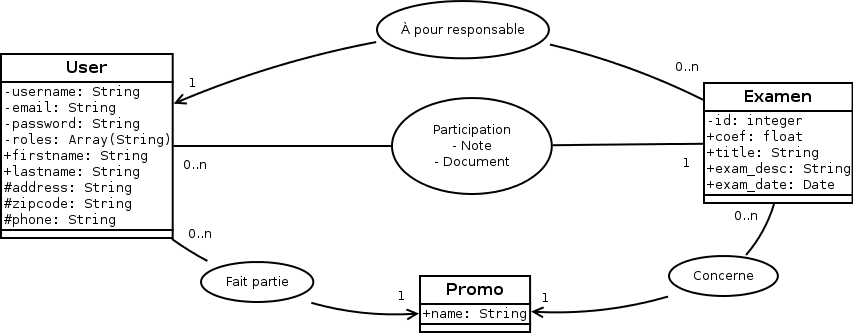
\includegraphics[width=0.9\textwidth]{./data.png}
    \end{figure}

    \begin{figure}
      \caption{Modèle physique de base de données}
      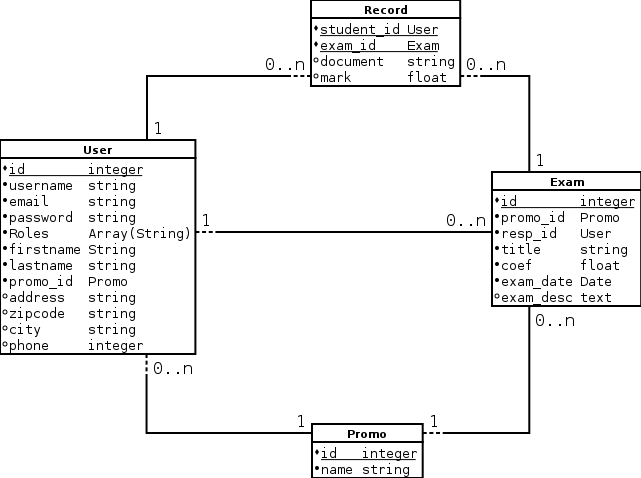
\includegraphics[width=0.9\textwidth]{./db.png}
    \end{figure}

    \subsection{User}
      En plus des champs prérequis :
      \begin{itemize}
        \item{Prénom}
        \item{Nom}
        \item{Adresse}
        \item{Code postal}
        \item{Ville}
        \item{Adresse e-mail}
        \item{Numéro de téléphone}
      \end{itemize}

      Le UserBundle nous rajoute toute la partie nécessaire à la gestion de
      l'utilisateur côté serveur.
      \begin{itemize}
        \item{Le mot de passe $\Rightarrow$ chiffré en sha1 dans la BDD}
        \item{Les rôles $\Rightarrow$ Pour la gestion des permissions}
        \item{Nom d'utilisateur}
        \item{Expiration du compte, confirmation par email etc.}
      \end{itemize}

      Et enfin nous avons ajouté un champ pour notre besoin qui est une
      promotion, en effet, on considère qu'un étudiant appartient à une
      promotion précise.

    \subsection{Promo}
      Les promotions correspondent à un regroupement d'utilisateur, dans le cas d'utilisation présent, tous les étudiants d'une même année 
      appartiennent à une promotion unique.

    \subsection{Exam}
      Un examen représente une épreuve définie par un enseignant. L'examen 
			comprend les propriétés suivantes :
			\begin{itemize}
				\item{Titre}
				\item{Descrption}
				\item{Promotion}
				\item{Coefficient}
				\item{Date limite}
				\item{Responsable : Un user responsable de TD}
			\end{itemize}
			Par défaut, lors de la création de l'examen, tous les étudiants de la promotion sélectionnée sont concernés par l'examen, mais il est également possible de modifier au cas par cas si un étudiant est affecté par l'examen.
    \subsection{Record}
			L'entité Record fait le lien entre les étudiants et les examens. En effet dans un record on attribue pour un étudiant et un examen, la note, ainsi que le document rendu (Fichier pdf ou word).

			On a donc :
			\begin{itemize}
				\item{Étudiant}
				\item{Examen}
				\item{Note}
				\item{Document}
			\end{itemize}

			Ainsi un Record avec la note et le document NULL, correspond au fait qu'un étudiant doit effectuer un rendu pour un tel examen. Quand il rend quelque chose, on peuple le champ 'Document'. Et ensuite quand l'examen est terminé le responsable de l'examen peut associer une note.


  \section{Réalisation Technique}
    \subsection{UserBundle}
      Nous avons utilisé un Bundle d'extension nommé : 
      \href{https://github.com/FriendsOfSymfony/FOSUserBundle}{UserBundle}.
      
      Ce bundle constitue la brique applicative qui permet d'effectuer toutes les actions nécessaires à presque tous les projets, c'est-à-dire :
      \begin{itemize}
        \item{Inscription}
        \item{Authentification}
        \item{Connexion}
        \item{Déconnexion}
        \item{Gestion du profil}
        \item{Changement de mot de passe}
      \end{itemize}
      Nous évitant du travail laborieux qui ne sert pas sur le plan métier de l'application.

    \subsection{Les tests avec PHPUnit}
			Nous avons principalement testé les différentes entités. Grâce à PHPUnit nous avons généré la couverture en tests de notre code.

			\href{http://ares-ensiie.eu/~unbekandt2011/UnsapaIPW/cov}{Couverture des tests}
    \subsection{La documentation développeur avec phpDocumentor}
			Tout notre code a été documenté en utilisant phpDocumentor. On peut trouvé cette documentation à l'adresse :

			\href{http://ares-ensiie.eu/~unbekandt2011/UnsapaIPW/doc}{Documentation développeur}

  \section*{Conclusion}
  \addcontentsline{toc}{section}{Conclusion}

\end{document}
